\documentclass[a4paper,12pt,titlepage]{article}
\pdfpagewidth
\paperwidth
\pdfpageheight
\paperheight



\usepackage[italian]{babel} 
\usepackage[T1]{fontenc} 
\usepackage[utf8]{inputenc} 
\usepackage{graphicx,color,listings}
\usepackage{fancyhdr} 
\usepackage{mathtools}
\usepackage{mhsetup}
\usepackage{amscd} 
\usepackage[usenames,dvipsnames]{xcolor}
\frenchspacing
\usepackage{geometry}
\usepackage{caption}
\captionsetup{labelformat=empty, textfont=sl}
\geometry{a4paper,tmargin=3cm,bmargin=3cm, lmargin=3cm,rmargin=2cm} \usepackage{multirow}

\textwidth16cm\textheight24cm\topmargin0mm\headheight0mm\headsep6mm\oddsidemargin0mm\evensidemargin0mm

\usepackage{siunitx}



\begin{document}
\author{David De Pol}
\title{Simulazione di scenari di scuotimento
sismico ad Ischia mediante l'utilizzo
della Web App XeRiS}
\maketitle
\tableofcontents
\clearpage

\section{Introduzione}

L'Italia è un'area ad elevata sismicità caratterizzata dalla presenza di numerose faglie sismicamente attive, situate nella litosfera a profondità relativamente               modeste. Si stima che nel passato esse abbiano provocato eventi 
sismici di magnitudo anche superiore a 7.0, come ad esempio il terremoto
calabro-siculo del 1908, che danneggiò gravemente le città di Reggio Calabria e Messina provocando più di novantamila morti.\\
La mappa italiana di pericolosità sismica (PCM 28 aprile 2006) segnala ampie porzioni del territorio nazionale su cui può incidere un importante fattore di rischio.

\begin{figure}[htbp]
 \centering
 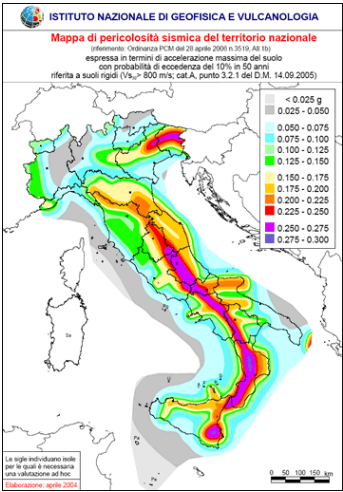
\includegraphics[width=.5\linewidth]{Img/PericolositaSismoNazionale.png}
 \caption{Mappa italiana di pericolosità sismica PCM 28 aprile 2006.}
 \label{fig:PericolositaSismoNazionale1}
\end{figure}

La pericolosità sismica è associata agli effetti fisici di un sisma che possono rivelarsi potenzialmente dannosi per l'uomo e/o le sue attività, come ad
esempio il massimo scuotimento orizzontale del suolo, solitamente espresso in PGA (Peak Ground Acceleration). Il rischio sismico, in sintesi, rappresenta
la probabilità che l'uomo, e/o le sue attività, subiscano un livello di danno se esposti a pericolosità sismica; viene valutato in concomitanza dei fattori di
pericolo, vulnerabilità ed esposizione. La vulnerabilità sismica indica la predisposizione di una costruzione a subire un determinato danno se soggetta a
un evento sismico di data entità, mentre l'esposizione descrive l'abbondanza di beni esposti al pericolo (e.g. vite umane, edifci e opere d'arte).\\
I livelli di scuotimento del suolo sono determinati principalmente dai seguenti fattori:\\

\begin{itemize}
\item  La magnitudo: indica la quantità di energia sismica rilasciata dal terremoto, ed è espressa in forma logaritmica. Tra un'unità di magnitudo e la
successiva corrispondono differenze energetiche circa di trentadue volte.
\item  La distanza epicentrale: si misura tra il sito in cui sono valutati gli effetti del sisma, e la porzione di litosfera dalla quale ha origine la rottura da cui si propagano le onde sismiche.
\item  Il processo di rottura: determina la direttività della rottura sul piano di faglia incidendo anche sulle caratteristiche del segnale sismico, percepito al sito.
\item  Le proprietà del mezzo attraversato dalle onde sismiche: gioca un ruolo fondamentale determinando i fattori di amplificazione e di decadimento
dei fronti d'onda.
\end{itemize}

Al fine di prevedere possibili scenari sismici può essere condivisibile l'idea di usare degli strumenti che permettano la simulazione di eventi sismici
realistici, basati su dati debitamente validati, misurati e/o stimati, caratterizzanti le sorgenti sismiche, i processi cinematici di rottura e gli effetti di sito.\\

In questo lavoro di tesi sono stati modellizzati eventi di scenari sismici ad Ischia, in corrispondenza della stazione sismica IOCA di Casamicciola, generati da sorgenti sismogeniche con caratteristiche tettoniche e ubicazioni geografiche differenti.\\
Gli eventi di scenario sono stati simulati utilizzando l'applicazione web XeRiS (Vaccari 2016), mentre i dati per la caratterizzazione delle sorgenti sismiche
sono stati tratti dal Database of Individual Seismogenic Sources (DISS Working Group, 2018).\\
Sono state prese in considerazione sei sorgenti sismiche: una situata sulla faglia di Casamicciola nella parte settentrionale dell'isola, le altre su alcune faglie appenniniche presenti nell'Italia meridionale, a una distanza di circa cento chilometri dal sito scelto.\\
Per quanto riguarda l'attribuzione delle caratteristiche geo-sismologiche utilizzate nella simulazione in cui la sorgente è posizionata sulla faglia di
Casamicciola, si è deciso di utilizzare quelle concernenti il terremoto di Casamicciola del 21 agosto 2017 (M=4), rilevate alla stazione sismica IOCA e
stimate da sismologi e geofisici. Tale decisione consegue dal fatto che è necessario mantenere sotto controllo il grado di consistenza tra le previsioni
ottenute e gli eventi sismici realmente accaduti. Non si avrà la pretesa di ottenere come risultato delle simulazioni dei livelli di scuotimento del suolo coincidenti a quelli effettivamente rilevati, ma una stima ragionevole di quanto ci si può attendere in futuro per eventi simili.\\
Si è deciso di simulare questo terremoto specifico poiché presenta delle caratteristiche particolari (e.g. De Natale, 2018), che possono essere approfondite al fine di dare un contributo alla stesura di nuove mappe di pericolosità per l'Isola d'Ischia più realistiche rispetto a quelle adottate dalla normativa nazionale attuale.\\
Il lavoro svolto è costituito di tre parti: nella prima sono presentate le funzionalità utilizzate dell'applicazione web XeRiS, e riportati i dati geosismologici relativi alla sorgete sismica di Casamicciola. Nella seconda parte sono presentati i risultati della simulazione con sorgente sull'isola, tabulate le faglie appenniniche e presentati i relativi scenari di scuotimento ad Ischia. Nella terza e ultima parte sono confrontati i diversi scenari di scuotimento simulati.

\section{Presentazione della Web App XeRiS}

XeRiS è un'applicazione web (in inglese Web App) (Vaccari, 2016), che permette la valutazione neo-deterministica della pericolosità sismica (Panza et al., 2001, Panza et al., 2012) mediante un'intuitiva interfaccia utente, nascondendo all'utente finale le complessità insite nel motore di calcolo.\\
Attraverso la simulazione di eventi sismici e il calcolo di scenari di scuotimento realistici, valutati in un singolo sito d'interesse o in un'area attorno all'epicentro, si possono calcolare i parametri di scuotimento del suolo, come ad esempio la Peak Ground Acceleration (PGA), tipicamente adottata per la stima della pericolosità sismica. Ma XeRiS genera anche le serie temporali, in spostamento, velocità ed accelerazione, che possono essere utilizzate dagli ingegneri come input sismico per la progettazione di strutture resistenti al sisma.\\
Con valutazione neo-deterministica della pericolosità, si intende che per la costruzione degli scenari di scuotimento sismico, si tengono in considerazione il modello della sorgente, le modalità di propagazione del segnale e gli effetti di sito, rispettando le leggi fisiche che descrivono la generazione e la propagazione delle onde sismiche.
\begin{figure}[htbp]
 \centering
 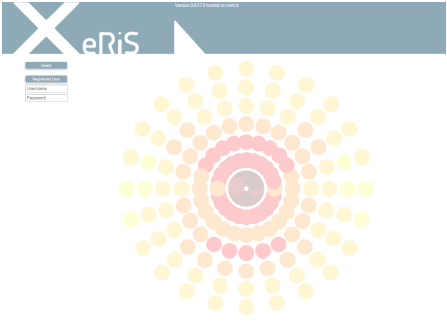
\includegraphics[width=.5\linewidth]{Img/XerisLogIn.png}
 \caption{Login XeRiS}
 \label{fig:Login XeRiS2}
\end{figure}
Inizialmente XeRiS richiede la definizione di un modello strutturale stratificato per la porzione di litosfera, nella quale noi collocheremo la faglia, in cui ha origine il processo di rottura e da cui si propagheranno i fronti d'onda del sisma. E' possibile selezionarne uno già implementato oppure utilizzarne di nuovi creati ad hoc.\\
Successivamente, si modellizza la sorgente sismica attribuendone le caratteristiche geo-sismologiche, nel nostro caso quelle disponibili nel Database of Individual Seismogenic Sources (DISS Working Group, 2018).\\
Per rappresentare al meglio la fisica del problema, la sorgente sarà considerata estesa, e dunque non trattata come un punto materiale posizionato in corrispondenza dell'ipocentro del terremoto, bensì approssimata ad una superficie rettangolare di dimensioni appropriate (e.g. Wells and Coppersmith, 1994), contenente al suo interno delle sotto-sorgenti che potranno essere considerate puntiformi.\\
Dopo aver scelto il sito d'interesse, nel caso in esame le coordinate della stazione sismica IOCA di Casamicciola sull'Isola d'Ischia, avrà luogo il calcolo dei segnali sismici che potranno essere utilizzati come input sismico.\\
In questo modo sarà generata una banca dati per un insieme di terremoti di scenario con caratteristiche tettoniche e ubicazioni geografiche differenti, utile per confrontare gli effetti ad Ischia dei diversi terremoti e quindi anche al fine di valutare quale evento sismico possa determinare una maggior pericolosità.
\clearpage

\subsection{Definizione del modello strutturale}
XeRiS utilizza la teoria della somma modale (Panza, 1985; Florsch et al., 1991) per il calcolo dei sismogrammi sintetici quando la distanza tra il sito d' interesse, cioè dove sarà valutato l'input sismico, e la sorgente del segnale è maggiore della profondità ipocentrale. Ciò accade nella maggior parte dei casi, mentre se tale distanza è minore interviene il metodo numerico DWN (Discrete Wave Number Technique) (Pavlov, 2009). La tecnica modale permette di ottenere dei sismogrammi accurati in maniera molto efficiente dal punto di vista computazionale, prendendo in considerazione anche l'attenuazione anelastica per la propagazione del segnale. Per poter applicare la teoria della somma modale, è necessario definire un modello di semispazio stratificato lateralmente omogeneo (1D), che esprime le caratteristiche medie della porzione di litosfera considerata, di cui XeRiS dovrà calcolare i modi di oscillazione per le onde di Rayleigh (campo P-SV) e di Love (campo SH). Ciascuno strato è caratterizzato dalle seguenti quantità (Fig.2.2): spessore, densità ($\rho$), velocità onde P e S (Vp e Vs) ed i fattori di qualità (inversamente proporzionali all'attenuazione) delle onde Vp e Vs, rispettivamente Qp e Qs. Per convenzione fisica, alla struttura deve essere garantita una profondità di \SI{100}{\kilo\metre} o \SI{1000}{\kilo\metre}, per calcoli rispettivamente su scala locale e regionale. XeRiS approssima la porzione litosferica senza prendere in considerazione la curvatura della superficie terrestre.

\begin{figure}[htbp]
 \centering
 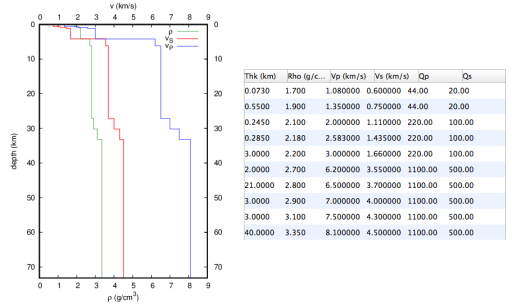
\includegraphics[width=.5\linewidth]{Img/ModelloStrutturaleIschia.png}
 \caption{Sinistra: densità (in verde) e velocità delle onde P ed S (blu, rosso)
in funzione della profondità. Destra: modello strutturale usato per Ischia.}
 \label{fig:ModStrIsc}
\end{figure}

Le onde sismiche di superficie che determinano il moto del suolo sono le onde di Love e di Rayleigh: si tratta di perturbazioni progressive che si propagano sulla superficie terrestre.\\
Le onde di Love sono caratterizzate da uno sforzo di taglio perpendicolare alla direzione di propagazione del fronte d'onda, mentre le onde di Rayleigh determinano un moto retrogrado ellissoidale del suolo, e decadono rapidamente all'aumentare della profondità (Fig.2.3). In Fig.2.4 sono rappresentati graficamente gli autovalori per i modi di Rayleigh e di Love della struttura ischiam0001 utilizzata per la simulazione con epicentro ad Ischia (De Natale et al., 2018).\\
Lo stesso modello stratificato viene utilizzato anche con la metodologia DWN, che se da un lato permette di considerare siti posizionati anche sulla verticale del piano di faglia, dall'altro risulta molto più onerosa dal punto di vista computazionale, maggiore è la distanza dall'epicentro e al crescere delle frequenze considerate nella generazione dei sismogrammi sintetici.

\begin{figure}[htbp]
 \centering
 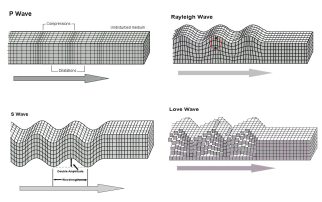
\includegraphics[width=.5\linewidth]{Img/PandSwaves.png}
 \caption{Rappresentazione grafica delle onde di corpo e di superficie.}
 \label{fig:PandSwaves}
\end{figure}

\begin{figure}[htbp]
 \centering
 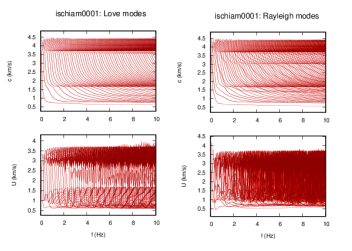
\includegraphics[width=.5\linewidth]{Img/IscModes.png}
 \caption{Rappresentazione grafica degli autovalori per i modi di  Love (a sinistra) e Rayleigh (a
destra) relativi alla struttura ischiam0001; In alto sono
riportate le velocità di fase (c), in basso le velocità di gruppo (U).}
 \label{fig:IscModes}
\end{figure}

\subsection{Modellizzazione di sorgenti sismiche estese}

Modellizzare una sorgente sismica estesa significa definire i suoi parametri geologici, tettonici e sismici che permettono di caratterizzarla: ubicazione, dimensioni ed orientazione del piano di faglia, meccanismo focale e processo cinematico di rottura. Tali fattori, unitamente alle proprietà del modello strutturale attraversato dalla perturbazione sismica, determineranno le caratteristiche del segnale sismico ottenuto al sito di interesse.\\
I parametri utilizzati nella simulazione dell'evento sismico con sorgente ad Ischia sono riportati in Fig.2.5.

\begin{figure}[htbp]
 \centering
 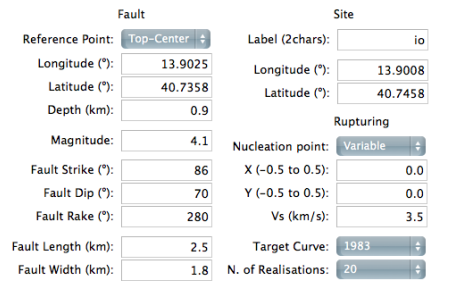
\includegraphics[width=.5\linewidth]{Img/Paratmeters.png}
 \caption{Dati specifici della sorgente situata sulla faglia di Casamicciola.}
 \label{fig:Paratmeters}
\end{figure}

I parametri che descrivono il meccanismo focale sono:
\begin{itemize}
\item  Fault strike: è l'angolo tra il nord magnetico indicato dall'ago della bussola e la linea di direzione della faglia, tale angolo si misura in senso
orario da \ang{0} a \ang{360}.
\item  Fault dip: indica l'angolo tra la faglia e il piano orizzontale, da \ang{0} a \ang{90}.
\item Fault rake: è la direzione del movimento dell' hanging wall durante il fenomeno di rottura, misurato rispetto il piano di faglia. Si misura relativamente al fault strike e assume valori da \ang{0} a \ang{360}.
\end{itemize}
%
Il processo di rottura viene considerato un fenomeno stocastico caratterizzato dal suo punto di nucleazione, dalla velocità di propagazione della frattura e da una specifica mappa di scorrimento della roccia sul piano di faglia (Fig.2.6).\\
Pertanto ai fini del calcolo del segnale sismico emesso sono prese in considerazione diverse modalità di scorrimento sul piano di faglia, per maggiori dettagli si rimanda il lettore al paragrafo seguente.\\
All'interno del rettangolo che approssima la faglia (Fig.2.7) si considera un sotto-rettangolo, nel quale è posizionato in modo casuale il punto di nucleazione dal quale ha origine il processo di rottura.\\
Attorno sono localizzate le sotto-sorgenti puntiformi disposte in modo ordinato su una griglia regolare, rappresentate in Fig.2.6 e in Fig. 2.7 come delle croci, che nel complesso simulano la sorgente estesa, mentre in bianco sono rappresentate le curve isocrone relative alla propagazione del processo di rottura.\\
Per tenere in considerazione anche un eventuale effetto analogo a quello Doppler in acustica, XeRiS valuta la direttività dei fronti d'onda in funzione del punto di nucleazione casuale, del meccanismo focale e del sito in cui si valutano gli effetti del input sismico.\\

\begin{figure}[htbp]
 \centering
 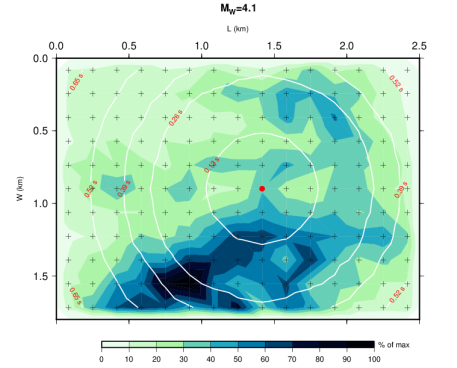
\includegraphics[width = 150pt, height = 150pt]{Img/SlipMap.png}
 \caption{Esempio di mappa di un processo di rottura: le diverse tonalità di colore esprimono le percentuali di scorrimento relativo dei blocchi di faglia, rispetto quello massimo rappresentato in nero. In rosso è raffigurato il punto di nucleazione (casuale) e in bianco le curve isocrone della propagazione della rottura.}
 \label{fig:SlipMap}
\end{figure}

\begin{figure}[htbp]%da mettere nella stessa page del img precedente
 \centering
 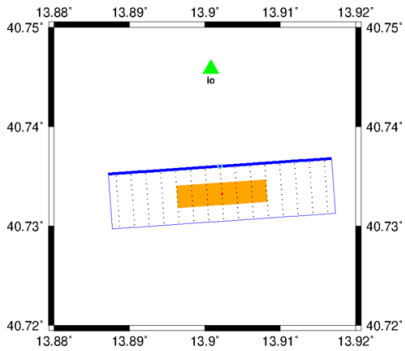
\includegraphics[width = 150pt, height =150pt]{Img/Positions.png}
 \caption{Posizione relativa del sito in cui è situata la stazione IOCA (io) e le coordinate in cui si trova la faglia. Il rettangolo arancione rappresenta il sotto rettangolo in cui può variare il punto di nucleazione casuale dal quale ha origine la rottura. I puntini blu rappresentano le sottosorgenti.}
 \label{fig:Positions}
\end{figure}
\clearpage

\subsection{Modellazione del moto del suolo generato da sorgenti sismiche estese}
Il segnale sismico generato da un modello di sorgente sismica estesa, si ottiene dalla combinazione dei segnali emessi da un insieme di sottosorgenti puntiformi, localizzate nel rettangolo che approssima la faglia.\\
Per studiare eventi sismici su scala locale, in altre parole per simulazioni in cui tra sorgente e ricevitore intercorre una distanza dell'ordine delle decine di chilometri, è necessario definire il modello strutturale fino a una profondità di un centinaio di chilometri ed è necessario impostare la frequenza di cut off a \SI{10}{\hertz}, poiché sulle brevi distanze il segnale sismico è dominato dalle alte frequenze.\\
All'aumentare delle distanze i segnali ad alta frequenza diventano sempre meno rilevanti, poiché intervengono fattori che determinano il decadimento della loro ampiezza d'onda.\\
Tra le principali cause dello smorzamento ci sono:\\

\begin{itemize}
\item  L'anelasticità del mezzo, che incide maggiormente su segnali ad alta frequenza che compiono più cicli.
\item Lo sparpagliamento geometrico, il fronte d'onda si amplia dunque le onde sferiche (onde di corpo) e cilindriche (onde di superficie) decadono in ampiezza rispettivamente come $\frac{1}{r}$ e $\frac{1}{\sqrt{r}}$.
\end{itemize}
%
Per scenari regionali, in cui le distanze sono dell'ordine anche delle centinaia di chilometri, si fissa la frequenza di cut off dell'input sismico a \SI{1}{\hertz} (poiché nel segnale sismico dominano le basse frequenze), infatti sulle lunghe distanze i segnali ad alta frequenza sono, relativamente, molto attenuati e in prima approssimazione il loro contributo può essere trascurato.
\clearpage

\subsection{Parametri di scuotimento del suolo}

I principali parametri per descrivere lo scuotimento del suolo sono:
\begin{itemize}
\item PGA Peak Ground Acceleration: valore del picco di accelerazione orizzontale del suolo, si ottiene dalla somma quadratica sotto radice del picco di accelerazione radiale e trasversale.
\item PGV Peak Ground Velocity: valore del picco di velocità orizzontale del suolo.
\item PGD Peak Ground Displacement: valore del picco di spostamento orizzontale del suolo.
\end{itemize}

Gli effetti della perturbazione sismica sugli edifici sono legati al loro periodo naturale di oscillazione.\\
Per studiare gli effetti del sisma su eventuali edifici presenti nel sito d'interesse, è possibile, in prima approssimazione, considerarli come dei pendoli unidimensionali rovesciati, con periodi di oscillazione crescenti.\\
Forzando tale sistema con un segnale sismico, cominceranno ad oscillare in modo differente in base alla frequenza propria di risonanza, determinata unicamente dalla lunghezza del pendolo con cui è approssimato l'edificio, ed in relazione al contenuto in frequenza del segnale sismico forzante.\\
Il valore in accelerazione massimo che si osserva per ciascun pendolo, prende il nome di accelerazione spettrale, che se graficato in funzione del periodo di oscillazione permette di ottenere il grafico dello spettro di risposta in accelerazione. Quindi è possibile associare a un'azione sismica esterna l'accelerazione massima a cui sono soggetti edifici con frequenze di risonanza diverse.\\
Data l'imprevedibilità del processo di rottura, ai fini del calcolo del segnale utilizzato come input sismico, sono prese in considerazione diverse modalità di scorrimento sul piano di faglia, quindi calcolato il segnale emesso e tracciato il grafico dello spettro di risposta per ciascuna realizzazione nel sito d'interesse.\\
Successivamente, XeRiS valuta periodo per periodo il cinquantesimo ed il novantacinquesimo percentile dell'accelerazione spettrale per l'insieme degli spettri di risposta ottenuti e traccia il grafico MCSI per l'unica sorgente considerata.\\
In questo caso particolare, la zona in grigio presente nel grafico MCSI, rappresenta l'area tra i percentili presi in considerazione.\\
Nel caso in cui ad un sito si vogliano valutare gli effetti sullo scuotimento del terreno (solitamente nel dominio dell'accelerazione) dovuti a sorgenti sismiche differenti per caratteristiche tettoniche e/o posizione geografica, è possibile considerare in uno stesso grafico MCSI gli spettri di risposta ottenuti per le varie sorgenti, con i relativi percentili.\\
Realizzando un tale grafico su XeRiS, appariranno in tabella solo le sorgenti che determinano un contributo dominante almeno in un periodo dello spettro.\\

\begin{figure}[htbp]%da mettere nella stessa page del img precedente
 \centering
 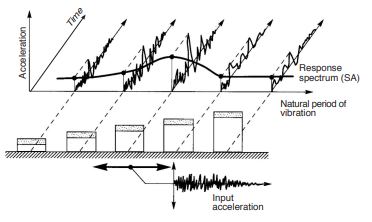
\includegraphics[width = 150pt, height =150pt]{Img/oscillatori.png}
 \caption{Costruzione del grafico dello spettro di risposta in accelerazione.}
 \label{fig:oscillatori}
\end{figure}

\begin{figure}[htbp]%da mettere nella stessa page del img precedente
 \centering
 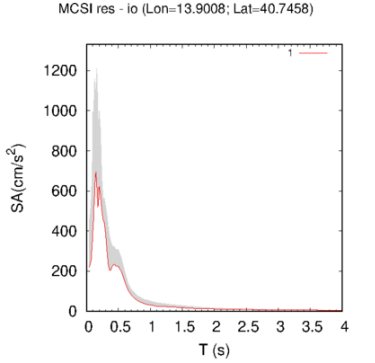
\includegraphics[width = 150pt, height =150pt]{Img/MCSI.png}
 \caption{Esempio di grafico MCSI per una singola sorgente, in grigio l'area tra il 50esimo e il 95esimo percentile.}
 \label{fig:MCSI}
\end{figure}
\clearpage

\subsection{Test parametrici}
XeRiS offre la possibilità di effettuare dei rapidi test parametrici: questo tipo di studio permette di analizzare come variano i valori di scuotimento del suolo, in funzione della variazione di un parametro libero scelto, caratterizzate la sorgente sismica.\\
Il test consiste nel fissare i parametri che caratterizzano la sorgente lasciandone variare solamente uno, entro un intervallo predefinito e con un passo scelto a piacere.\\
Per ogni valore che assume la variabile libera, saranno elaborati dei sismogrammi sintetici, che verranno poi utilizzati come input sismico, per ottenere il grafico dell'accelerazione radiale, trasversale e verticale del moto del suolo in funzione del parametro libero. L'accelerazione radiale e trasversale sono le componenti vettoriali dell'accelerazione orizzontale del moto del suolo.\\
Occorre specificare che in questa funzionalità di XeRiS, la faglia non è considerata estesa, ma viene approssimata ad una sorgente puntiforme opportunamente scalata nello spazio (SSPS - Size Scaled Point Source) o semi estesa,
ovvero scalata nello spazio e nel tempo (STSPS - Size and Time Scaled Point Source) (Panza et al., 2012), a discrezione dell'utente.\\
Per prima cosa è necessario definire il modello strutturale in cui noi posizioneremo la faglia e dove si propagheranno le onde sismiche.\\
Successivamente, si inseriscono i parametri fissi, si seleziona il parametro libero, si specifica il range di variabilità e lo step di variazione.\\
Infine si seleziona il modello di sorgente. Se si decide di approssimare la sorgente come puntiforme (SSPS), essa rappresenta una dislocazione istantanea della roccia sul piano di faglia. In alternativa è possibile selezionare un modello di sorgente semi estesa (STSPS) già implementato, oppure prepararne di nuovi ad hoc nel pannello Sources, specificandone poi il tipo di rottura (unilaterale o bilaterale), la direttività di propagazione della rottura sul piano di faglia se si osserva il fenomeno dal sito d'interesse, e il numero di realizzazioni con cui si vuole simulare tale evento.
\clearpage

\section{Simulazione di eventi di scenario}
\subsection{Simulazione del terremoto a Ischia: Faglia di Casamicciola}
\subsection{ Simulazione di eventi di scenario ad Ischia per sorgenti appenniniche}
\subsection{Confronto tra alcune simulazioni con sorgente appenninica}

\section*{Conclusioni}\addcontentsline{toc}{section}{Conclusioni}

\end{document}